\chapter{Experiments and Results}\label{chapter:experiments} 
In this chapter, an empirical investigation into the structure of winning tickets is conducted.
First, the datasets that were used are described in detail.
Then, experiments were conducted that attempt to find separate subnetworks in the winning ticket, for both datasets.
Finally, the connectivity of the network to the network input is examined.

\section{Datasets}
\textcite{BIMT} conducted experiments on symbolic regression datasets.
These are simple toy datasets where the labels are computed with a symbolic formula. 
For instance regarding the independence task, the inputs are $x_1, x_2, x_3, x_4$ and the outputs are $y_1={x_2}^2 + \sin{(\pi*x_4)}$ and $y_2={(x_1+x_3)}^3$.
In this case, the independence is obvious, as $y_1$ depends only on $x_2$ and $x_4$, and $y_2$ depends only on $x_1$ and $x_3$.
However, concerning the lottery ticket hypothesis, the existing literature focuses on classification tasks, while this is a regression task.
Therefore instead of using the independence dataset from \textcite{BIMT}, 
two classification datasets that contain independent tasks are created in the scope of this thesis, which are described in the following sections.

\subsection{Moons-Circles Dataset}\label{sec:independece_dataset}
The first dataset is a combination of two classic toy datasets, which are concatenated into one dataset.
The two selected datasets are the Two-Moons dataset and the Circles dataset, depicted in figure~\ref{fig:moons_circles}.
Both datasets can be interpreted as a two-dimensional plane, where the inputs describe the coordinates of points on the plane. 
The labels of the dataset relate to the class, either red or blue.

\begin{figure}
\centering 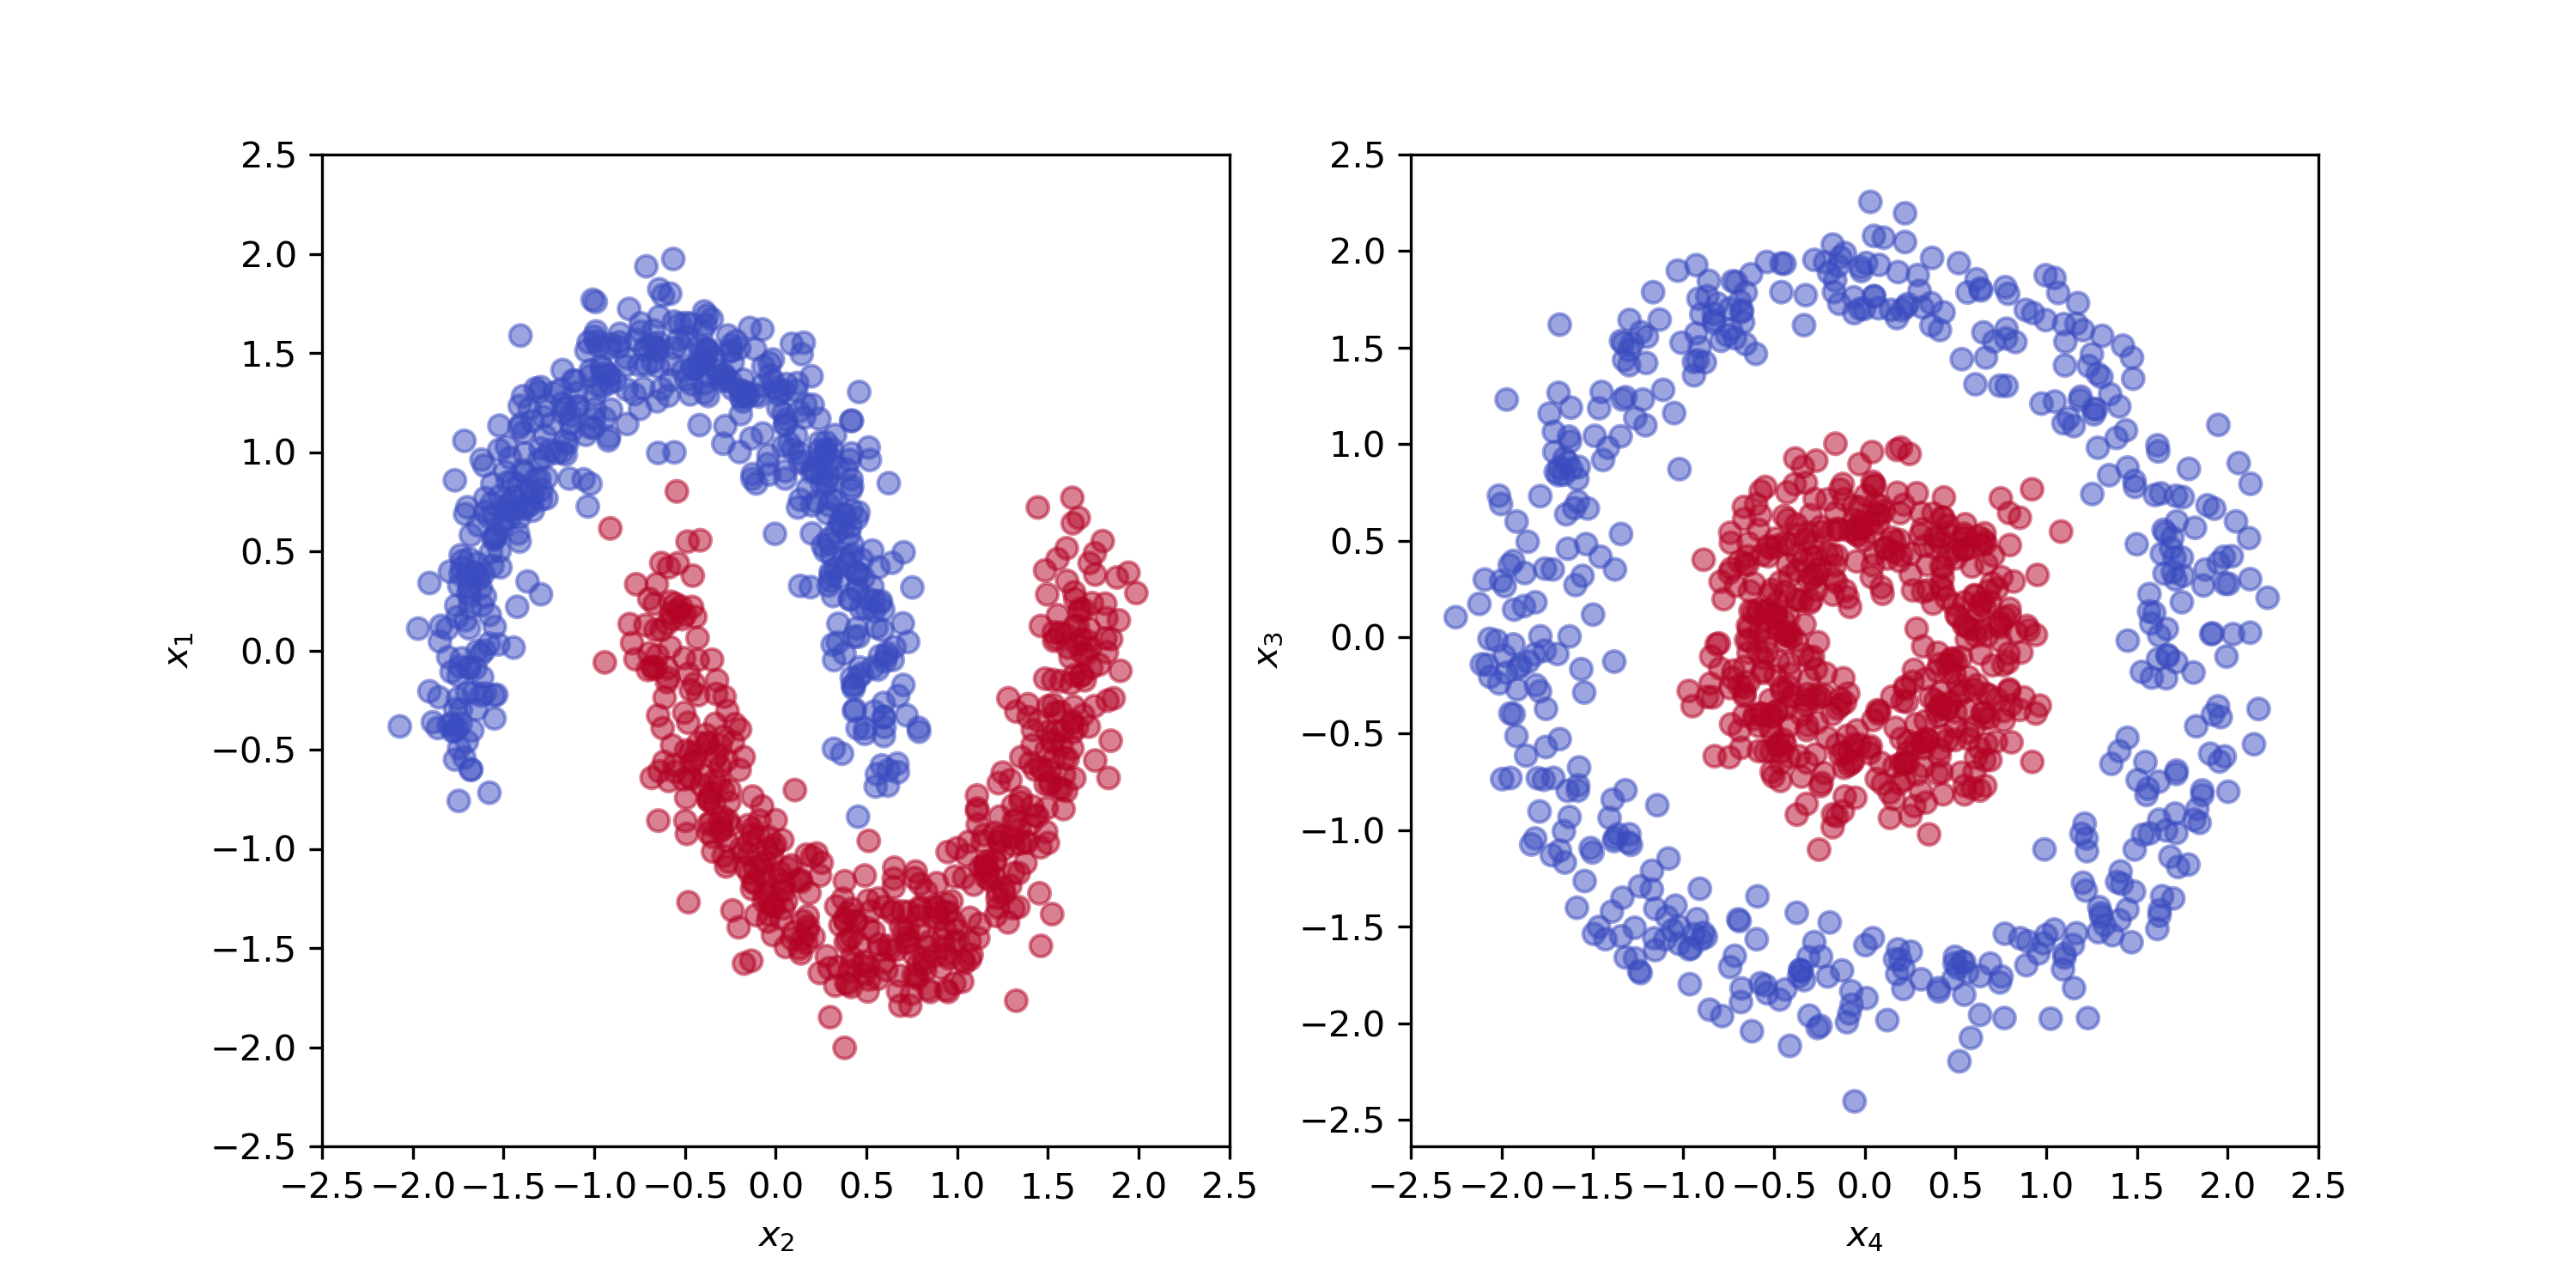
\includegraphics[width=1.0\linewidth]{moons-circles.png}
\caption[Two-Moons and Circles Dataset]{
    The Two-Moons dataset (left) and the Circles dataset (right); normalized to zero mean and unit variance.}\label{fig:moons_circles}
\end{figure}

Concretley, let $( x_1 , x_2 )$ be the inputs of the Two-Moons dataset and $y_1 \in \{0,1\}$ the class label.
The samples are generated by creating two half circles of evenly spaced points, with a radius of one.
One of the half circles is rotated by 180 degrees and shifted by $0.5$.
Gaussian noise with a mean of zero and standard deviation of $0.1$ is added to each point in the dataset.
Let $( x_3 , x_4 )$ be the inputs of the cirlces dataset and $y_2 \in \{0,1\}$ the class label.
The data is generated by creating evenly spaced points on the inner and outer circles. 
The center of both circles is at $(0,0)$ and the radius of the outer circle is one.
The radius of the inner circle is set to be $0.35$.
Gaussian noise with a mean of zero and standard deviation of $0.1$ is added to each point in the dataset.
The values of noise and the size of the inner circle are selected, such that the points do not mix among the circles.

\begin{figure}[t]
\centering
\begin{minipage}{\linewidth}
\begin{lstlisting}[
    language=Python,
    captionpos=b, 
    label={code:data},
    caption={[Dataset Generation]Generation of Moons-Circles dataset with scikit-learn~\autocite{sklearn}; pseudo code},
]
from sklearn import make_circles, make_moons
from sklearn.model_selection import train_test_split

# generates shuffled data points with labels
# x1, x2 -> shape=(1000, 2); y1, y2 -> shape=(1000, ) 
x1, y1 = make_circles(n_samples=2000, noise=0.1, factor=0.35)
x2, y2 = make_moons(n_samples=2000, noise=0.1)

circles_moons_x = concatenate(x1, x2) # shape=(1000,4)
circles_moons_y = concatenate(y1, y2) # shape=(1000,2)

# split the dataset in half
x_train, x_test, y_train, y_test = train_test_split(
    circles_moons_x, circles_moons_y, test_size=0.5
)

# scale data to zero mean, unit variance, based on training data
scaler = sklearn.preprocessing.StandardScaler().fit(x_train)
x_train = scaler.transform(x_train)
x_test = scaler.transform(x_test)

(x_train, y_train) # the training data
(x_test, y_test) # the test data
\end{lstlisting}
\end{minipage}
\end{figure}

The classic machine learning library Scikit-Learn~\autocite{sklearn} is used to generate the data. 
The code snippet~\ref{code:data} outlines the generation process as Python-flavoured pseudo code.
The previously described sampling strategies for the data relate to the implementation in the Scikit-Learn Python library.
The data is generated with the \lstinline{makemoons}, and \lstinline{makecircles} functions, respectively.
Since the ranges of values of the datasets are different due to their sampling strategy, each feature is normalized individually to have zero mean and unit variance.
The final, normalized datasets are depicted in figure~\ref{fig:moons_circles}

To create a single dataset out of the two separate datasets, the input features as well as the labels are concatenated.
Concretely, one sample of the concatenated dataset $\hat x$ contains one randomly selected sample from the Two-Moons dataset and one randomly selected sample from the Circles dataset.
The label $\hat y$ of the sample $\hat x$ also consists of the respective concatenated labels.
\[\hat x = ( x_1 , x_2 , x_3 , x_4 )\]
\[\hat y = ( y_1 , y_2 )\]
In this way, the whole dataset is concatenated.
Afterward, the dataset is randomly split in half into a training set and a test set.
The result is a training set and a test set with 1000 samples each.
This dataset contains two separate and independent tasks.
For each task, only the respective inputs contain valuable information for the prediction of the class.

\begin{figure}[t]
    \centering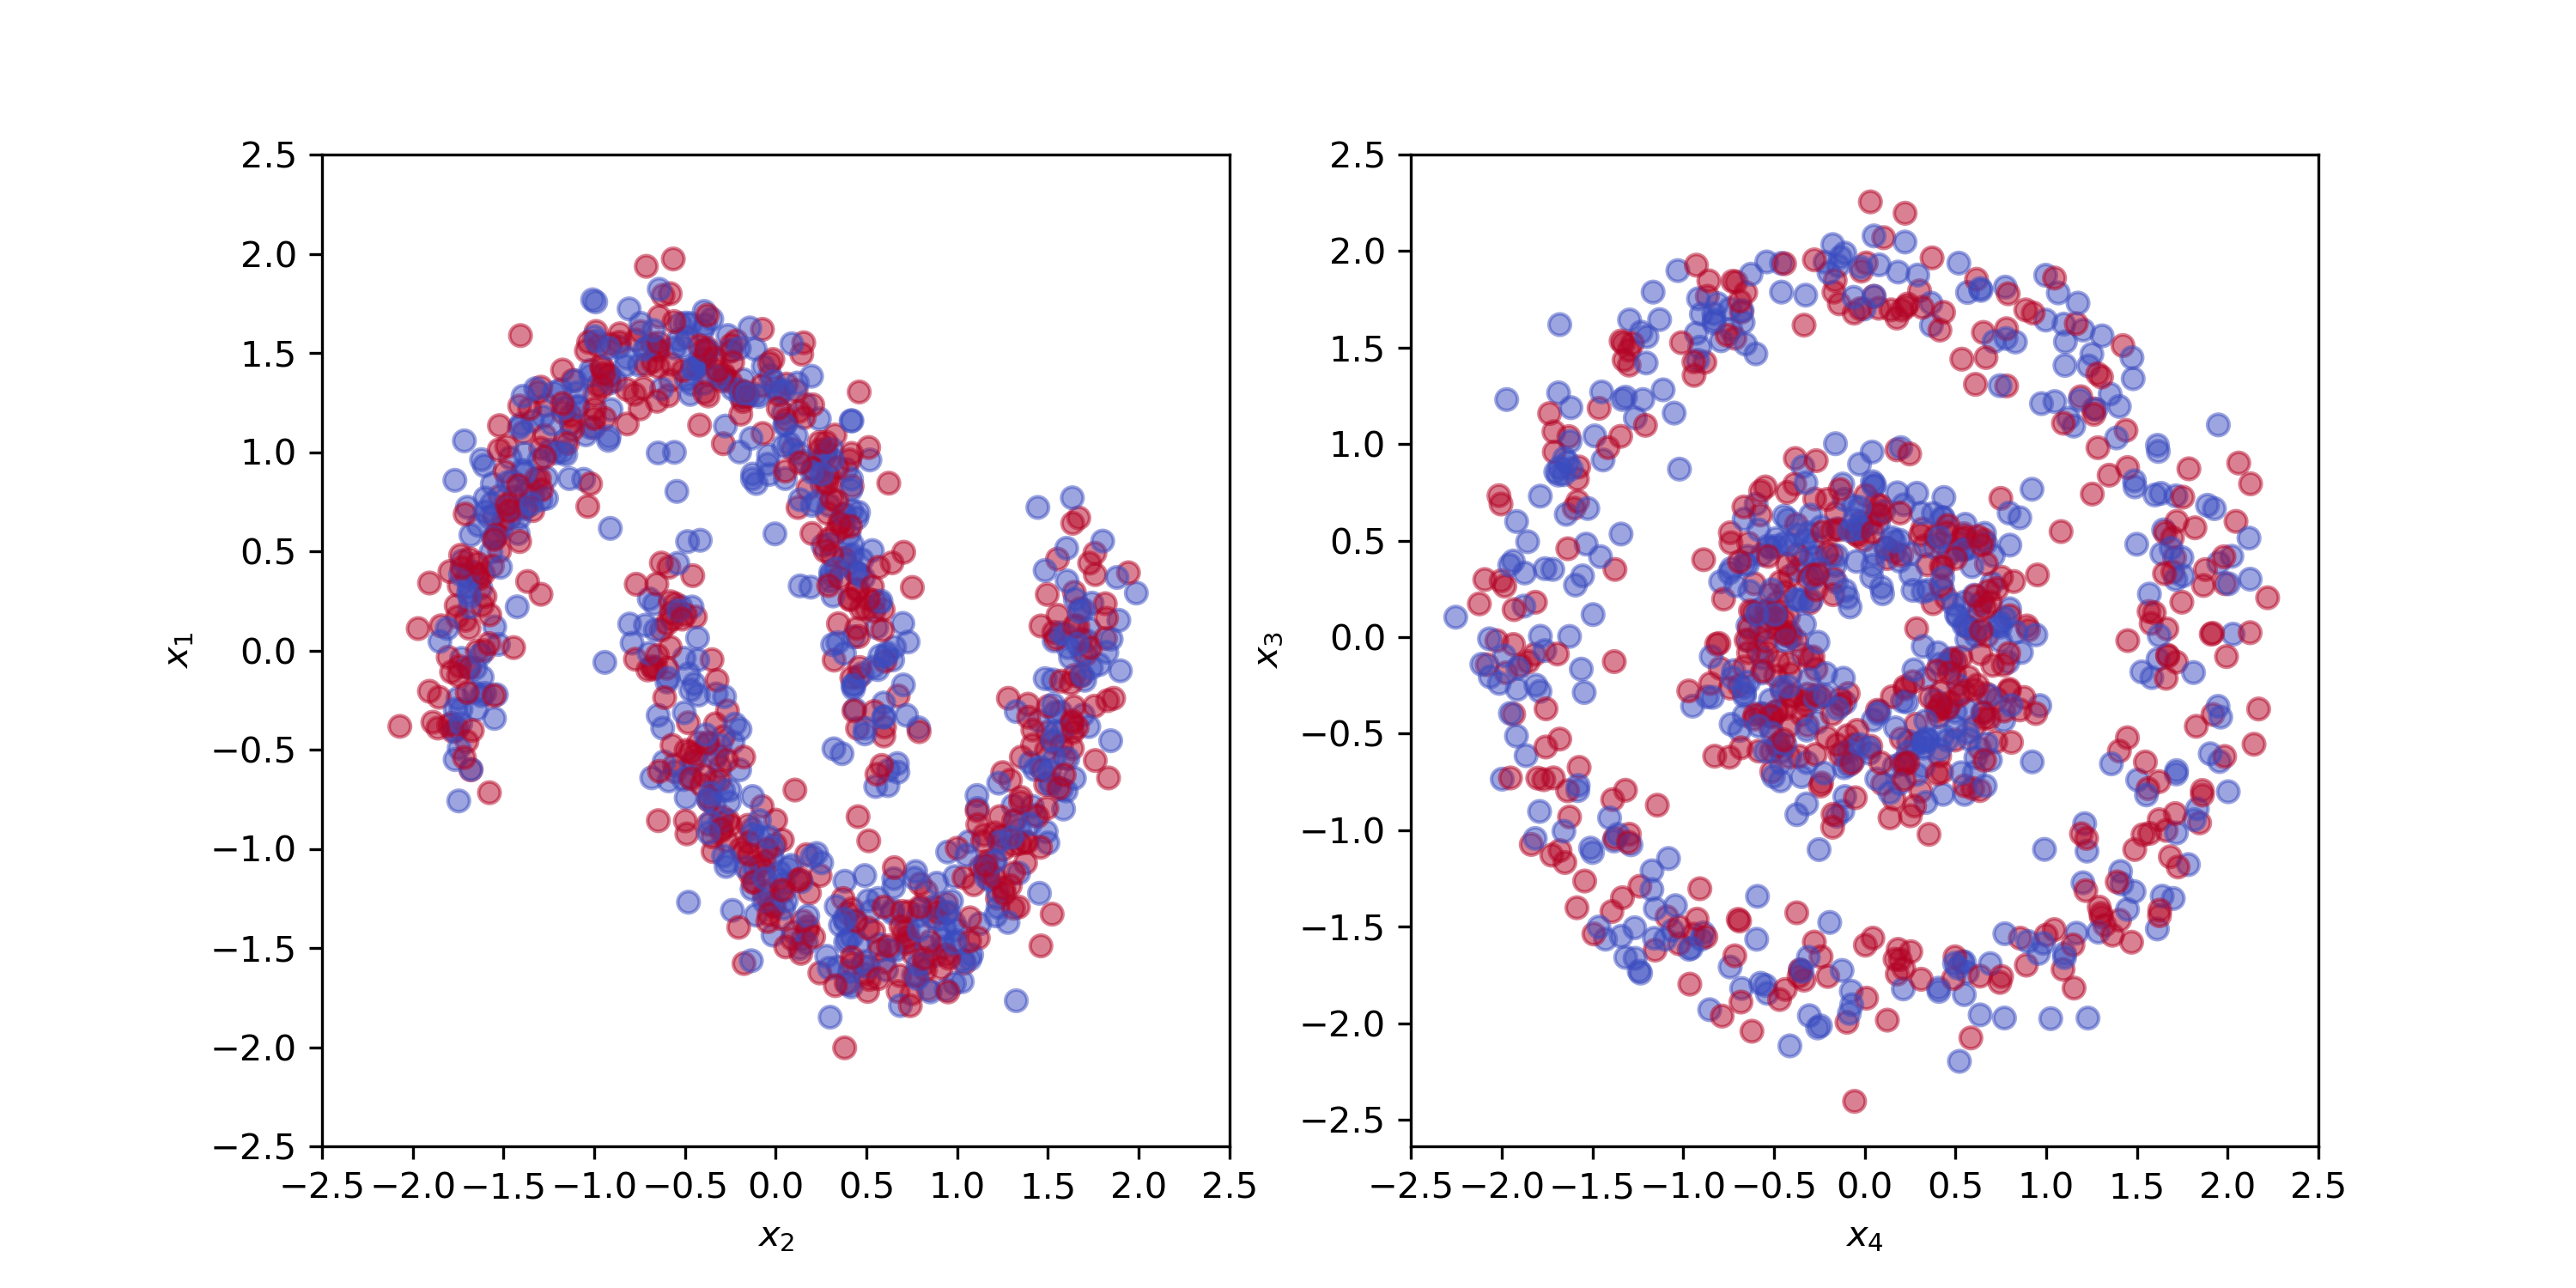
\includegraphics[width=1.0\linewidth]{moons-circles-inverted.png}
    \caption[Two-Moons and Circles Dataset, inverted labels]{
        The Two-Moons dataset (left) with Circles labels, and the Circles dataset (right) with Two-Moons labels. 
    }\label{fig:moons_circles_inverted}
\end{figure}

The independence is demonstrated in figure~\ref{fig:moons_circles_inverted}.
The dataset is the same as is visible in figure~\ref{fig:moons_circles}. 
However, the Two-Moons dataset is displayed with the labels of the Circles dataset and vice versa.
Concretely, on the left side, the coordinates represent $x_1$ and $x_2$, but the colors refer to $y_2$.
On the right side on the other hand, $x_3$ and $x4$ are displayed with the colors defined by $y_1$.
There is no clear visible pattern discernible from these datasets given on their own.

The generation procedure of the datasets is outlined in the Python-flavoured pseudo code snippet~\ref{code:data}.
First, both datasets are individually generated.
The samples and labels are then concatenated into one dataset, which is then randomly split into the training and test set.
Finally, the data is normalized to zero mean and unit variance, based on the training set.
The generated dataset will be referred to as the \textit{Moons-Circles} dataset.

\subsection{MNIST-Fashion-MNIST Dataset}\label{sec:mnist}
To test the network separation on a slightly more realistic problem, the MNIST-Fashion-MNIST dataset is created.
The dataset is created similarly to the Moons-Circles dataset described in paragraph~\ref{sec:independece_dataset}, but the MNIST dataset~\autocite{mnist} and the Fashion-MNIST~\autocite{fashion} dataset are used as tasks.
The MNIST dataset is a well-known dataset of handwritten digits. 
The training set consists of 60000 images and the test set of 10000.
It contains all digits from zero to nine in handwritten form, on a $28 \times 28$ pixel grayscale image.
This dataset was also used in the original lottery ticket experiments by~\textcite{LTH}.

\begin{figure}[t]
    \centering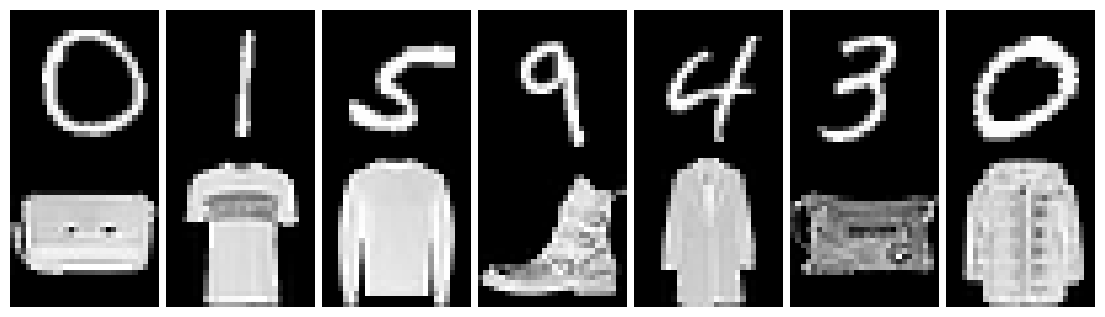
\includegraphics[width=1.0\linewidth]{mnist-fashion-mnist.png}
    \caption[MNIST-Fashion-MNIST dataset]{
        The MNIST-Fashion-MNIST dataset; Each sample contains a random MNIST image (top) and a random Fashion-MNIST image (bottom).
    }\label{fig:mnist_fashion}
\end{figure}

As the name suggests, the Fashion-MNIST dataset~\autocite{fashion} is similar to the MNIST dataset.
However, instead of handwritten digits, different items of clothing are displayed on the $28 \times 28$ grayscale image.
It contains the same number of images for the test set and the training set.
Both datasets contain 10 classes.
In the same way as described in paragraph~\ref{sec:independece_dataset}, the datasets are concatenated into one.
Both datasets are shuffled and each sample from the MNIST dataset is concatenated with a random sample from the Fashion-MNIST dataset.
The class labels are also concatenated.
The result is a dataset with 60000 training samples and 10000 evaluation samples.
Through the concatenation, each image has an aspect ratio of $28 \times 56$, where each half corresponds to one of the datasets.
In figure~\ref{fig:mnist_fashion}, seven randomly selected samples of the  MNIST-Fashion-MNIST dataset are displayed.
On the top of each image, the handwritten MNIST digit is displayed. 
On the bottom the fashion item is visible.
Each sample consists of one random digit and one random fashion item. 

Contrary to the previous task, this dataset contains significantly more input features.
Each dataset has 784 input features, which results in 1586 input features for the concatenated dataset.
The Moons-Circles dataset only has four input features and two output features.
Further, the previous task was a combination of two binary classification tasks.
Now, each dataset represents a multiclass classification problem with 10 classes.

\newpage
\section{Experiments on the Moons-Circles Dataset}
The first round of experiments is dedicated to finding out what conditions are required, such that the network separates when trained on the Moons-Circles dataset.
During a preliminary exploration phase, some scenarios where the network indeed separates were found.
Yet, they were sparse and could not be easily interpreted.
Therefore, in this step, the knowledge gained from the initial experiments was put to use.
A systematic evaluation of the relationship between network size and splitting behavior was conducted.

To enable comparison between networks of different sizes, the network extension technique described in paragraph~\ref{sec:extension} was used.
First, an extensive experiment with a base network architecture of $(4,8,8,2)$ was conducted.
To expand the range of the results, two additional experiments were conducted, which were slightly smaller to lower computational cost.
One experiment is done on a network with only one hidden layer, concretely with a shape $(4,20,2)$, and the other experiment on a network with three hidden layers, a shape of $(4,4,4,4,2)$.
All other hyperparameters are shared among the three experiments.
The only difference is the pruning target, which is derived from the network architecture.

For all three experiments, the pruning rate was set to $0.32$.
The chosen value, while somewhat arbitrary, was selected by promising results on preliminary tests.
\textcite{LTH} used a pruning rate of $0.2$ in the original experiments for the fully connected feed-forward network trained on the MNIST dataset.
However, with a larger pruning rate, a larger space of network sizes can be covered with the same number of iterations, which is why the larger pruning rate of $0.32$ was selected.

\subsection{Exploring Network Architectures - Model Extension}\label{two-hidden}
The first experiment architecture that is discussed is the network with two hidden layers.
The base network, which is the network that is used as a base for extending, has the shape $(4,8,8,2)$.
This architecture has 112 weights, which is also used as the pruning target.
The network architecture indicated by the number of neurons per hidden layer and the respective number of weights are displayed in table~\ref{tab:trajectory}.
The network is extended up to 25 times.
At the extension level 25, the network has a shape of $(4,1310,1310,2)$, with 1.723.960 weights.
The number of extension levels corresponds to the number of pruning levels the network goes through.
After each pruning level, the network is evaluated to check if it is separated or degraded.

When considering all pruning levels, there are four different scenarios for a network:
\begin{enumerate}
\item \textbf{Separated:}
The network separates at some pruning level. 
It does not degrade at any later level. 
\item \textbf{Separated-Degraded:} 
The network splits at some point and has all input and output nodes.
At a later level, the network degrades (it loses at least one input or output).
\item \textbf{Degraded:} 
The network degrades before it can separate.
\item \textbf{Interconnected:} 
The network does neither separate nor degrade. 
The result is a single network that contains all input and output nodes of all tasks.
\end{enumerate}

\begin{table}[t]\scriptsize
    {
    \sffamily
    \caption[Parameter Trajectories of different network sizes]{
    In this table, the parameter trajectories and the corresponding hidden dimension of the network are displayed for each extension level. 
    The parameter trajectory is in each respective `param' column and the number of hidden neurons per hidden layer is in the column `hidden'.
    At the extension level zero, the base model values are displayed.
    }\label{tab:trajectory}
    \begin{tabular}{rrrrrrr}
    \toprule
    Lvl & hidden-1 & param-1 & hidden-2 & param-2 & hidden-3 & param-3 \\
    \midrule
    0 & 20 & 120 & 8 & 112 & 6 & 108 \\
    1 & 29 & 174 & 10 & 160 & 8 & 176 \\
    2 & 43 & 258 & 13 & 247 & 10 & 260 \\
    3 & 64 & 384 & 16 & 352 & 12 & 360 \\
    4 & 94 & 564 & 20 & 520 & 15 & 540 \\
    5 & 138 & 828 & 25 & 775 & 19 & 836 \\
    6 & 202 & 1212 & 31 & 1147 & 23 & 1196 \\
    7 & 297 & 1782 & 38 & 1672 & 29 & 1856 \\
    8 & 437 & 2622 & 47 & 2491 & 35 & 2660 \\
    9 & 643 & 3858 & 57 & 3591 & 43 & 3956 \\
    10 & 946 & 5676 & 70 & 5320 & 52 & 5720 \\
    11 & 1391 & 8346 & 85 & 7735 & 63 & 8316 \\
    12 & 2046 & 12276 & 104 & 11440 & 77 & 12320 \\
    13 & 3009 & 18054 & 127 & 16891 & 94 & 18236 \\
    14 & 4425 & 26550 & 154 & 24640 & 114 & 26676 \\
    15 & 6507 & 39042 & 188 & 36472 & 139 & 39476 \\
    16 & 9569 & 57414 & 229 & 53815 & 169 & 58136 \\
    17 &   &   & 278 & 78952 &   &   \\
    18 &   &   & 337 & 115591 &   &   \\
    19 &   &   & 410 & 170560 &   &   \\
    20 &   &   & 498 & 250992 &   &   \\
    21 &   &   & 604 & 368440 &   &   \\
    22 &   &   & 733 & 541687 &   &   \\
    23 &   &   & 890 & 797440 &   &   \\
    24 &   &   & 1080 & 1172880 &   &   \\
    25 &   &   & 1310 & 1723960 &   &   \\
    \bottomrule
    \end{tabular}
    }
\end{table}

\begin{figure}[t] % Stacked Area d=2
    \centering
    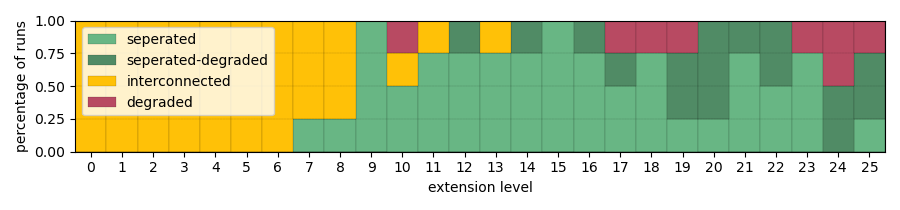
\includegraphics[width=1.0\linewidth]{2-layer-histogram-split-behaviour.png}
    \caption[Separation/Degradation Stacked Area Chart (2 hidden layers)]{
        A proportional stacked area chart showing the ratio of training runs in each category.
        The x-axis shows the extension level, and the y-axis shows the relative amount of networks in each category, stacked. (2 hidden layers)
        }\label{fig:2laxer-histogram}
\end{figure}

At each extension level, the runs are repeated with four different seeds for the network initialization.
The results are displayed in figure~\ref{fig:2laxer-histogram}.
The figure is a proportional stacked area chart, where each scenario described above is encoded with a color.
On the x-axis, the extension levels are shown.
On the y-axis, the percentage of networks in each category can be viewed.
A clear pattern in the data is, that the networks separate for the first time with at least 7 pruning levels.
The shape and number of weights at that level are $(4,38,38,2)$ and 1672 respectively, which is $\sim15$ times the number of weights compared to the base model. 
Starting at shape $(4,57,57,2)$ or extension level 9, which represents an increase of $\sim32$-times, the majority of the networks separate.
Up until the 6th extension level, none of the networks separate or degrade. 
However, if the network were pruned further, at some point every network would degrade eventually.
Therefore it is also reasonable to assume that some of the networks that are still interconnected after all pruning iterations would separate if they were pruned to a lower pruning target.

Another interesting observation is that only after extension level 10 the networks begin to degrade.
What follows from the data is the more extension levels, the more likely it is that a network degrades, either before or after it separates.
One possible explanation for this is that at each pruning level, a certain number of weights are made inactive.
As noted in \autocite{HanEtAl15, AllAlivePruning}, this is a known phenomenon.
However, since no regularization is used in these experiments, the inactive weights do not decrease in magnitude.
Rather, they are frozen with their last value.
If more inactive parameters are created at each pruning level than pruned, the percentage of inactive weights in the network grows with every iteration.
Therefore, the more pruning levels the network experienced, the less of its available, unpruned parameters are active.
This effectively makes the network smaller, which in turn makes it more likely to separate or degrade.

\begin{figure}[ht] % Less active more pruning
    \centering
    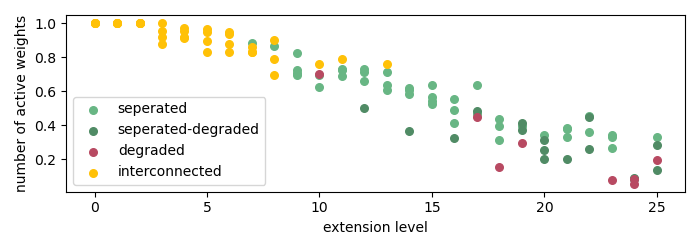
\includegraphics[width=1.0\linewidth]{2-layer-compund-damage.png}
    \caption[Correlation extension levels and rate of active weights]{
    The correlation between the number of extension levels and the percentage of active weights in the network.
    Each dot is a single training run, the colors indicate the category of the training run. (2 hidden layers)
    }\label{fig:collateral_damage}
\end{figure}

This effect is visualized in figure~\ref{fig:collateral_damage}.
The colors are encoded in the same way as in figure~\ref{fig:2laxer-histogram}.
Each dot represents a single training run. 
On the x-axis, the extension level is displayed.
On the y-axis, the number of active weights after the last pruning level is displayed.
A clear pattern emerges, showing a correlation between the number of pruning iterations and the number of active weights in the final network.
Important to note is that when a network degrades (red), the run is immediately stopped.
Therefore in this graph, the degraded networks might have larger numbers of active weights, compared to other networks that were pruned for the total amount of levels.
However, even with this caveat, a clear trend is visible.
The more pruning levels the network experiences, the smaller the percentage of the active network weights.
For some networks that were extended to 20 or more levels, the final percentage of active weights in the network is only $\sim20$ percent, which translates to only $\sim22$ active weights.
Techniques like L1-Regularisation used in \autocite{HanEtAl15} or All-Alive-Pruning \autocite{AllAlivePruning} could counteract this effect of compounding inactive parameters.
However, this is a topic for future research and is not addressed further in this thesis. 

To gain a broader picture of the effects shown on the network with two hidden layers, the same experiments were conducted on networks with one and three hidden layers.
Similar effects can be seen for these architectures.
As shown in table~\ref{tab:trajectory}, the networks were only extended for 16 levels instead of 25, to reduce computational requirements. 
As the networks get larger and the number of pruning levels is higher, the computational effort increases significantly.
For the network with one hidden layer a base network with shape $(4,20,2)$ was selected.
It has a similar number of weights compared to the base network with two layers.
\begin{figure}[t] % Stacked Area d=1
    \centering
    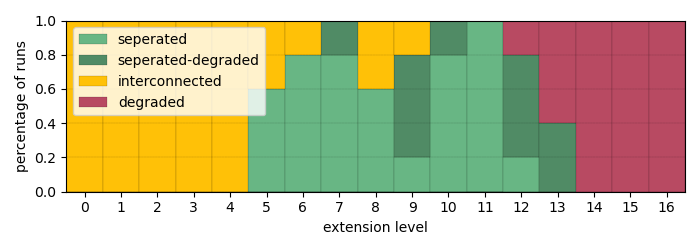
\includegraphics[width=1.0\linewidth]{1-layer-histogram-split-behaviour.png}
    \caption[Separation/Degradation Stacked Area Chart (1 hidden layer)]{       
        A proportional stacked area chart showing the ratio of training runs in each category.
        The x-axis shows the extension level, and the y-axis shows the relative amount of networks in each category, stacked; (1 hidden layer)
        }\label{fig:1layer-histogram}
\end{figure}

In figure~\ref{fig:1layer-histogram}, the same plot as for the two-layer experiment is presented.
On the x-axis, the extension level is displayed. 
Along the y-axis, the percentage of runs per category is shown.
Each color determines the category that the training run belongs to.
A similar trend is visible as in figure~\ref{fig:2laxer-histogram}.
After a certain number of pruning levels and at a certain network size, the networks begin to consistently separate.
Given a few more pruning levels, the networks start to degrade more often, either before or after they separate.
Interestingly, at extension level 12, the network starts to degrade more often before it separates.
Beginning at 14 extension levels, where the networks are the largest, they never separate and only degrade.
The reason for this behavior is unknown.
It might be that the networks with more hidden layers also exhibit such behavior at even higher extension levels. 

Regarding the network with three hidden layers, the results are similar.
\begin{figure}[t] % Stacked Area d=3
\centering
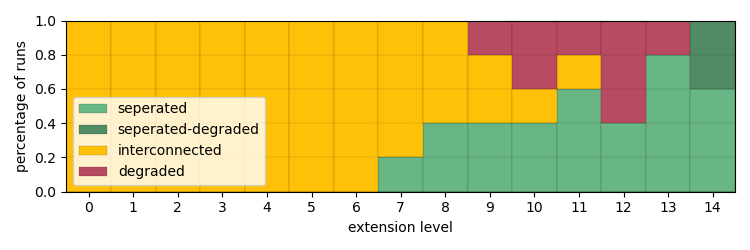
\includegraphics[width=1.0\linewidth]{3-layer-histogram-split-behaviour.png}
\caption[Separation/Degradation Stacked Area Chart (3 hidden layers)]{
A proportional stacked area chart showing the ratio of training runs in each category.
The x-axis shows the extension level, and the y-axis shows the relative amount of networks in each category, stacked. (3 hidden layers)
}\label{fig:3layer-histogram}
\end{figure}
In figure~\ref{fig:3layer-histogram} the same graph for the three-layer network is shown.
A similar effect occurs but unlike the single-layer network, the network does not stop to separate in the range that was tested. 

%%%%%%%%%%%%%%%%%%%%%%%%%%%%%%%%%%%%%%%

\subsection{When Do Networks Separate?}
Do the networks always start to separate at the same pruning level or with the same number of unpruned parameters?
This question is investigated in the following paragraph.
Interestingly, when extending the network to higher levels, it tends to separate into earlier pruning levels.
This results in an increased number of available weights to the network at the iteration they separated.
\begin{figure}[t] % Active/Available d=2
    \centering
    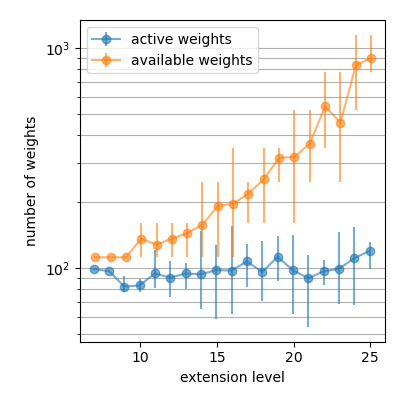
\includegraphics[width=.6\linewidth]{2-layer-active-available-at-split-log.png}
    \caption[Comparing active and available weights (2 hidden layers)]{
    The number of active weights (blue) and the number of available weights (orange).
    Each dot is an average of four training runs.
    The error bars indicate the minimum and maximum of the runs.
    Log scale. (2 hidden layers)
    }\label{fig:2l-active-split}
\end{figure}
Figure~\ref{fig:2l-active-split} depicts the number of available/unpruned weights in orange and the number of active weights in blue, for the different extension levels of networks with two hidden layers.
Each dot represents the average number of active or available weights at the exact iteration where the network is separated.
Only training runs where the network separates are taken into account.
For each extension level, the training run was repeated with four different seeds for the initialization of the network weights.
On the x-axis, the extension level of the network is displayed, which is also the number of pruning levels the network goes through.
The more extension levels, the larger the network.
The error bars indicate the maximum and minimum values of the different runs.
The graph is shown on a logarithmic scale.

A visible trend is the exponential increase of the number of available weights at the level where the network separates (orange).
This comes from the fact that the networks separate in earlier iterations, where there are more available weights.
Interestingly, the number of active weights does not experience comparable growth when the network is extended more.
Active weights are the weights that are contained in the active subgraph $\mathcal{G}_a$, that was introduced in chapter~\ref{chapter:method}.
It increases slightly but almost remains flat, covering a narrow range of around $80$ to $120$ weights, while the available weights grow from $120$ to around $900$.
This data indicates that the number of active weights might be an important quantity to network separation.
Since the active subgraph $\mathcal{G}_a$ is indeed the graph that is used to evaluate network separation, this seems plausible.
 
% 1 hidden layer
\begin{figure}[t] % Active/Available d=1
    \centering
    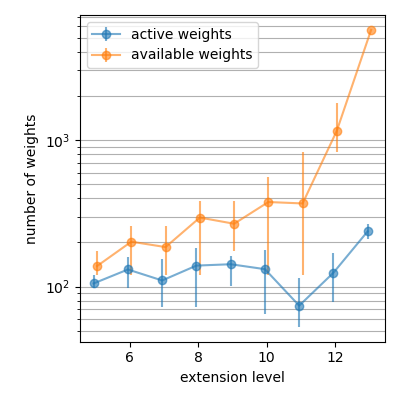
\includegraphics[width=0.6\linewidth]{1-layer-active-available-at-split-log.png}
    \caption[Comparing active and available weights (1 hidden layer)]{
    The number of active weights (blue) and the number of available weights (orange).
    Each dot is an average of four training runs.
    The error bars indicate the minimum and maximum of the runs.
    Log scale.  (1 hidden layer)
}\label{fig:1layer-active}
\end{figure}

When looking at the graph of the architectures with one hidden layer, this effect is even more dramatic, which is shown in figure~\ref{fig:1layer-active}.
Similarly to the experiment with two layers, the networks separate in earlier iterations when they are larger and have more pruning levels.
The number of active weights remains in a fairly tight range between $70$ and $120$ active weights, while the number of available weights goes from around $125$ to over $1400$.
Notably, as shown in figure~\ref{fig:1layer-histogram}, the network does not separate anymore after the 13th extension level.
At the 13th level, only around $10$ percent of the weights in the network are active at the separation iteration.

\begin{figure}[t] % Active/Available d=1
    \centering
    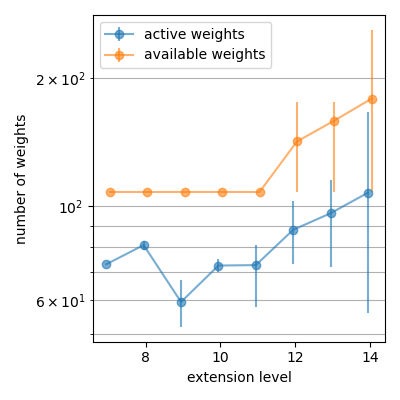
\includegraphics[width=0.5\linewidth]{3-layer-active-available-at-split-log.png}
    \caption[Comparing active and available weights (3 hidden layers)]{
    The number of active weights (blue) and the number of available weights (orange).
    Each dot is an average of four training runs.
    The error bars indicate the minimum and maximum of the runs.
    Log scale.  (3 hidden layers)
    }\label{fig:3layer-active}
\end{figure}

When considering the network with three hidden layers, a similar effect is visible, however significantly less pronounced.
Figure~\ref{fig:3layer-active} depicts the number of active weights and the number of available weights of the three-layer architectures with different extension levels.
The networks at extension level 7 until 11 all split at the last pruning level, which can be deducted by the number of available parameters which is equal to the pruning target of 108.
The number of active weights is slightly lower than in the other experiments.
The data indicates that separating a three-layer network with the same number of available parameters is less likely than a two or a one-layer network because the number of available weights does not grow as quickly.
Also when looking at the number of active weights at the level where the three-layer networks separate, the numbers are significantly lower compared to the other architectures.

\subsection{What Makes Networks Separate?}
As seen in figure~\ref{fig:2laxer-histogram}, the networks with two hidden layers start to split at 7 extension levels and a network shape of $(4,38,38,2)$, with 1672 weights.
However, it is not obvious what the main contributor to network separation is.
To gain a better understanding of that phenomenon an experiment was conducted that compares different combinations of pruning levels, network size, and pruning rate for the two-layer architectures.
For this experiment, four architectures were selected.
One network with shape $(4,31,31,2)$ (extension level 6), which did not separate in any run.
Networks with $38$ and $48$ hidden neurons (extension levels 7 and 8), where only one in four networks separated.
And finally a network with 57 hidden neurons, where all four runs have separated.
This range of architectures is assumed to encompass a critical area, due to the change in separation behavior.
Further, each of the four architectures was trained with $0$ to $10$ pruning levels.
The pruning target is fixed at $112$, such that all networks end up at the same number of unpruned parameters after the last pruning level.
Therefore, the pruning rate is variable depending on network size and number of levels.
The larger the network, the higher the pruning rate, given a fixed number of iterations.
Each training run with a combination of network size and number of pruning levels was repeated four times, with different seeds for the network initialization.

\begin{figure}[ht] % what influences separation : size
    \centering
    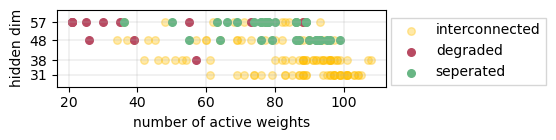
\includegraphics[width=1.0\linewidth]{grid-2-layer-eval-abs.png}
    \caption[Influence of network size on separation]{
        The influence of network size on separation is shown.
        Each dot is a single training run, color-coded by category.
        }\label{fig:grid-1}
\end{figure}

In figure~\ref{fig:grid-1} the impact of network size is demonstrated.
On the y-axis, the size of the network is encoded by its hidden dimension.
On the x-axis, the number of active weights after the last pruning level is depicted.
Each dot represents one training run.
The colors denote if the network separated, degraded or remained interconnected.
Regarding the two smaller networks with hidden dimensions $31$ and $38$, none of the networks separated. 
Increasing the number of pruning levels and decreasing the pruning rate did not result in separated networks.
On the other hand, the two larger networks separate numerous times.
These results indicate, that there is a phase change in the ability of the network to separate.
A certain level of overparameterization seems to be necessary for the network to separate well.

\begin{figure}[ht] % what influences separation : plevels
    \centering
    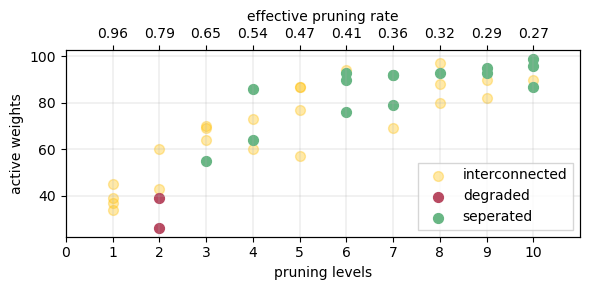
\includegraphics[width=1.0\linewidth]{grid-2-layer-pruning-rate-48-hd.png}
    \caption[Influence of pruning rate on separation]{
        Influence of the pruning rate on separation is shown.
        Each dot is a single training run, color-coded by category.
    }\label{fig:grid-2}
\end{figure}

To investigate the influence of pruning levels and pruning rate, the separation behavior of the network with hidden dimension 48 is depicted in figure~\ref{fig:grid-2}.
Since the pruning target and the network size are fixed, the pruning rate has to change when increasing the number of pruning levels.
On the bottom x-axis, the number of pruning levels is depicted, and on the top x-axis, is the corresponding pruning rate.
On the y-axis, the number of active weights after all pruning levels is depicted.
With more pruning levels and a lower pruning rate, the network is more likely to separate.
Also, a seemingly contradicting trend to figure~\ref{fig:collateral_damage} is visible, namely that the number of active weights increases with more pruning levels.
The difference to the previous experiment is, that while the number of pruning levels increases in both cases, the pruning rate decreases with more pruning levels in this experiment, which is visible in figure~\ref{fig:grid-2}. In the experiment depicted in figure~\ref{fig:collateral_damage}, the pruning rate is constant, while the network size increases.

However, this data also indicates that there is a certain phase change in the likelihood of the network separating.
Since the pruning rate and the number of pruning levels are two tightly interlinked parameters, it is hard to examine them in isolation.
The largest pruning rate where a network separated was $\sim0.65$. 
With pruning rates lower than $\sim0.41$, the networks consistently separate.
The data indicates that more pruning levels with lower pruning rates are generally favorable to network separation.
\textcite{LTH} already note that iterative pruning leads to smaller lottery tickets than one-shot pruning.
It is reasonable to assume, that the same phenomenon takes place concerning network separation.
Less pruning levels versus lower pruning rates represent a trade-off between favorable conditions and computational cost.

\subsection{How Do Networks Separate?}
Another open question is, what the process of separation looks like.
In the beginning, when the network is fully connected, it is not yet clear which weight and neuron belongs to which task.
One available option, however, is to view the network from the perspectives of the inputs and outputs.
The input and output features are the only parts of the network that can already be associated with a task when it is fully connected.
This enables determining the degree to which the neighboring layers have separated as well.

For instance, regarding the simple Moons-Circles dataset, there are two output neurons.
Each neuron in the penultimate layer has two outgoing connections: one to the Circles-output and one to the Moons-output.
When one of the connections is pruned, the neuron and all its incoming connections are automatically part of the task the unpruned weight is connected to.
The number of neurons in any given layer that are only connected to one of the outputs of one task is denoted $N_{decided}$.
The number of neurons that are connected to both tasks is denoted $N_{undecided}$.
The degree of separation is determined by 
\[ \frac{N_{decided}}{N_{decided}+N_{undecided}} \]
This calculation can be done from either the side of the inputs or the outputs and it works in the same way.
Only if a layer has at least one neuron that has \textit{decided} to which task it belongs, neurons in the next layer can \textit{decide} as well.

\begin{figure}[t] % Layer separation from outputs
    \centering
    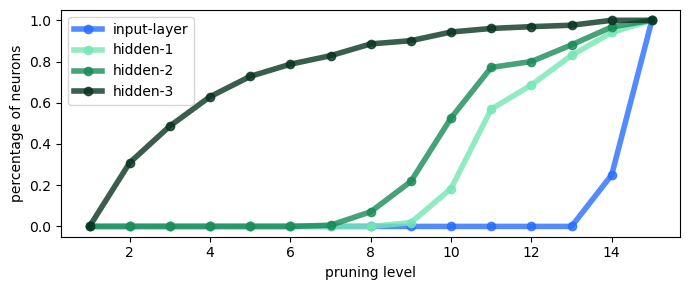
\includegraphics[width=0.9\linewidth]{output-view.png}
    \caption[Separation from the view of output neurons]{
    The degree to which neurons in hidden layers can be attributed to a task over the pruning levels; calculated by the connectivity to the output neurons.
    Each line shows the percentage of weights attributable to a task.
    The x-axis shows the pruning levels from 0, where the network is fully connected to 15, where the network separated.
    }\label{fig:outview}
\end{figure}

\begin{figure}[t] % Layer separation from inputs
    \centering
    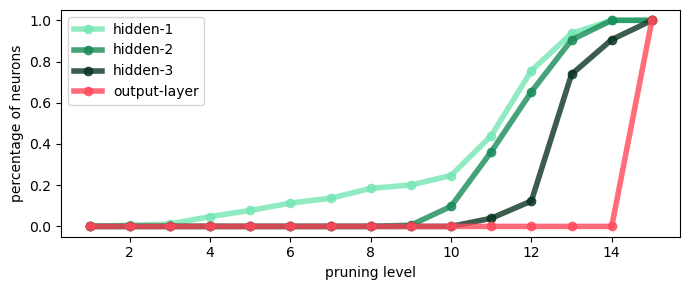
\includegraphics[width=0.9\linewidth]{input-view.png}
    \caption[Separation from the view of input neurons]{
        The degree to which neurons in hidden layers can be attributed to a task over the pruning levels; calculated by the connectivity to the input features.
        Each line shows the percentage of weights attributable to a task.
        The x-axis shows the pruning levels from 0, where the network is fully connected to 15, where the network separated.
    }\label{fig:inview}
\end{figure}

In figure~\ref{fig:outview} the degree of separation is displayed for each layer from the view of the outputs.
On the x-axis, the pruning levels are displayed and on the y-axis the percentage of neurons that can be attributed to a task.
The network in this case was taken from the experiment with three hidden layers.
It separates at iteration 15.
In the first iteration, none of the layers were separated.
Already by the second iteration, around $30$\% of the neurons in the last hidden layer (hidden-3) belong to only one task.
This increase in the degree of separation of this layer resembles a logarithmic growth.
At iteration 7, where already $\sim80$\% of neurons in the last hidden layer belong to a task, the penultimate hidden layer (hidden-2) starts to separate.
With one iteration delay, the next hidden layer (hidden-1) starts to separate.
It tracks the layer \textit{hidden-2} in its rapid, s-curve-shaped growth.
Only at iteration 14, when over $90$\% of neurons are already attributable to a task, the input layer separates.
In this case, the separation describes the perspective from the outputs.
It does not take into account the knowledge, of which input neuron belongs to which task.

The same network but from the view of the inputs is displayed in figure~\ref{fig:inview}.
On the x-axis, the pruning levels are displayed and on the y-axis the percentage of neurons that can be attributed to a task.
In this case, the separation is significantly slower in the beginning.
After iteration 10, the separation speeds up at iteration 15, the network is completely separated.
The difference in the degree of separation, depending on the point of view, could have several reasons.
It could be that the slower separation is due to the fact, that there are four inputs and only two outputs.
Therefore, for the neurons to be only connected to the inputs of one task, two instead of one weights have to be pruned.
Another possibility is that the weights in the first layer are higher in magnitude than the weights in the last layer.
This would result in stronger pruning in the last layer.

\subsection{Performance of Separated Networks}
One remaining question is if the networks still perform well when they separate.
Are they better, equal, or worse in terms of the validation loss, compared to the other networks?

\begin{figure}[t]
    \centering
    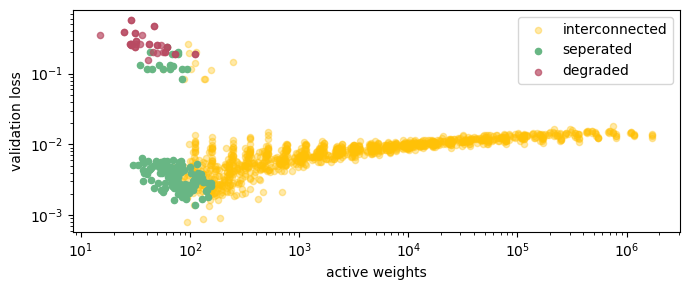
\includegraphics[width=0.9\linewidth]{performance.png}
    \caption[Performance of winning tickets]{
        The performance of winning tickets, color-coded by category.
        Winning tickets that separated are shown in green.
        Log scale. (2 hidden layers)
    }\label{fig:performance}
\end{figure}

To investigate the performance, the validation loss from the experiment with two hidden layers described in paragraph~\ref{two-hidden} was used.
In figure~\ref{fig:performance}, the validation loss is depicted on the y-axis.
On the x-axis, the number of active weights is displayed.
On the y-axis, the validation loss is shown.
Each dot represents a network at one stage.
An experiment with 20 pruning levels is shown with 20 dots in this figure.
The color refers to the state of the network at the iteration.
The color of the point represents if the network was interconnected (yellow), separated (green), or degraded (red) at the iteration the point refers to.
The loss value is calculated after the training and before the pruning of each iteration, as shown in the code snippet~\ref{code:imp}.

The bending line of yellow points demonstrates the consistent performance of the networks during the early iterations.
Likely due to early stopping, the networks remain at a validation loss of around $0.01$.
The loss decreases slightly over the pruning iterations.
A visible cluster of green dots sits at the end of the yellow line.
These dots represent the networks that are separated.
The iterations where the networks are separated are amongst the networks with the lowest loss.
This indicates that the separation of the networks is not merely a consequence of pruning to extremely high sparsities.
Rather, the separated networks still represent a well-performing function, even amongst the best-performing networks overall.

Interestingly, there is a second distinct cluster of networks.
It sits at the same number of active weights, however with significantly higher loss.
This cluster contains interconnected, separated, and degraded networks at seemingly even ratios.
Since the experiments were stopped as soon as a network degraded, the red points refer to losses immediately after the network degraded.
Even though the cluster looks compact along the y-axis it covers a fairly large range between 0.08 and 0.56 loss. These losses correspond to an accuracy of roughly $95$\% and $65$\% respectively.
The separated and interconnected networks still generally inhabit an area with lower loss than the degraded networks.

\subsection{Inactive Parameters and Zombies}
As introduced in chapter~\ref{chapter:method}, there are four different kinds of states the parameters of the network can be in.
Parameters can be pruned, inactive, active or zombies.
The number of pruned parameters increases at a predictable rate over the training run.
How do the other kinds of parameters evolve?
With the two-layer architectures extended over several levels as shown in table~\ref{tab:trajectory}, the inactive and zombie parameters are investigated.

\begin{figure}[t]
    \centering
    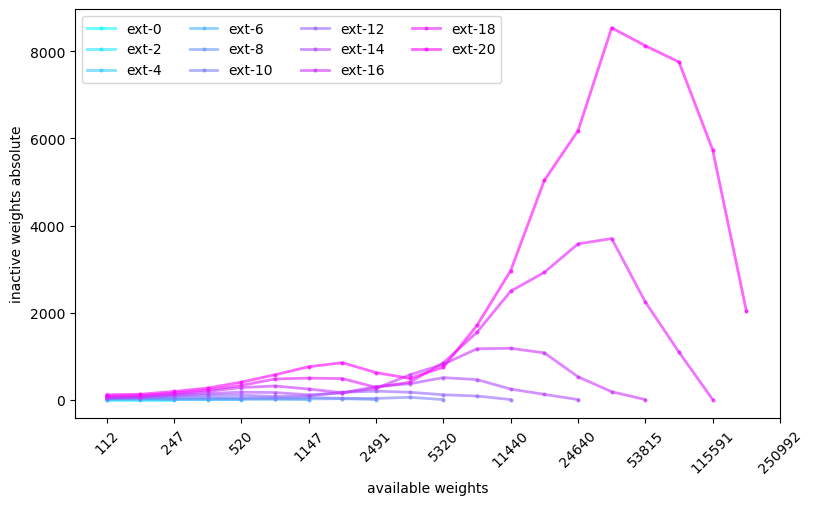
\includegraphics[width=.9\linewidth]{inactive-abs-2l.png}
    \caption[Inactive Weights during training runs, absolute]{
        The number of inactive weights over the training runs. 
        Each line represents a different extension level. 
        The x-axis shows the available weights and the y-axis shows the absolute number of inactive weights.
    }\label{fig:inactive-abs}
\end{figure}

In figure~\ref{fig:inactive-abs}, the absolute number of inactive weights is displayed.
Every line represents a certain network size, indicated by the extension level (ext-$i$).
Further, the lines are averages of four training runs with different seeds for model initialization.
On the x-axis, the number of available parameters of the network is displayed.
On the y-axis, the number of inactive weights in the network is shown.
Networks that were extended to higher levels, experienced more pruning levels and therefore have longer lines in the graph.
It is visible, that the number of inactive weights is larger with larger networks.
Especially at the earlier pruning iterations of each network, the numbers grow and subsequently fall significantly.
However, due to the reduction in the overall network size, this is to be expected.

\begin{figure}[t]
    \centering
    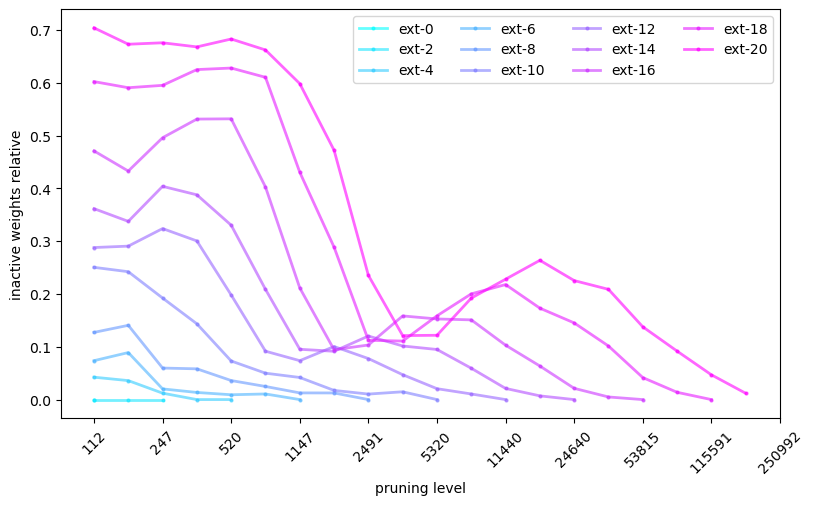
\includegraphics[width=.9\linewidth]{inactive-rel-2l.png}
    \caption[Inactive Weights during training runs, relative]{
        The number of inactive weights over the training runs. 
        Each line represents a different extension level. 
        The x-axis shows the available weights and the y-axis shows the relative number of inactive weights.
        }\label{fig:inactive-rel}
\end{figure}
The same graph, however with the relative amount of inactive weights is shown in figure~\ref{fig:inactive-rel}.
Here, a different trend is visible.
As the number of weights in the network decreases, the percentage of inactive weights generally increases.
Interestingly, this increase is not steady.
With larger network sizes, a distinct pattern emerges.
The ratio of inactive weights increases to a certain level and subsequently decreases, which results in a visible bump in the line.
Afterward, the value increases again until it flattens off.
The larger the network, the larger the number of inactive weights at the final pruning levels.
With smaller networks, this pattern cannot be seen.

\begin{figure}
    \centering
    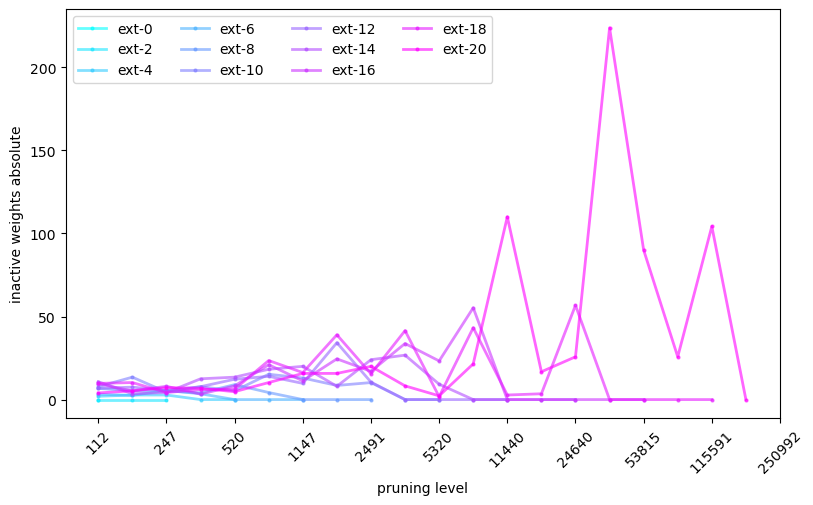
\includegraphics[width=.9\linewidth]{zombie-abs-2l.png}
    \caption[Zombie weights during training runs, absolute]{
    The number of zombie weights over the training runs. 
    Each line represents a different extension level. 
    The x-axis shows the available weights and the y-axis shows the absolute number of zombie weights.
    }\label{fig:zombie-abs}
\end{figure}

When examining the number of zombie weights in the network, a different pattern is visible.
In figure~\ref{fig:zombie-abs}, the absolute number of zombie weights is displayed for the same networks.
Similarly to figure~\ref{fig:inactive-abs}, the number of zombies is larger when the networks have more parameters available.
However, the number of zombie weights is significantly less than the number of inactive weights.

\begin{figure}
    \centering
    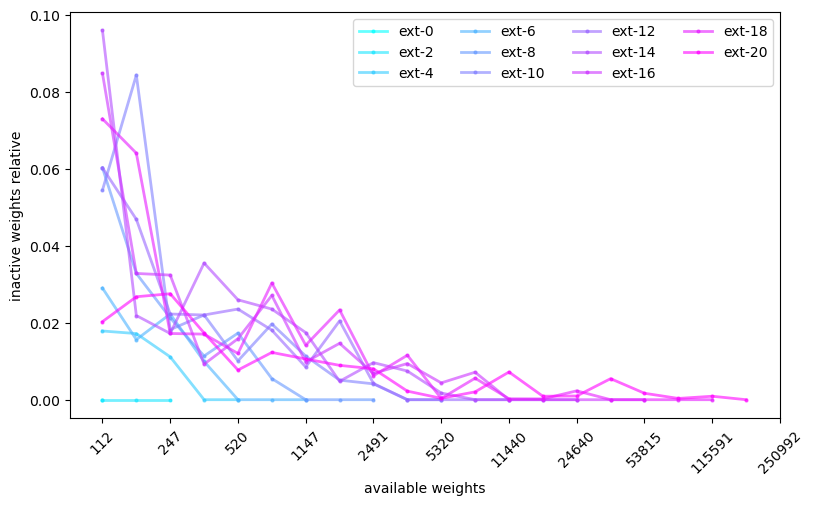
\includegraphics[width=.9\linewidth]{zombie-rel-2l.png}
    \caption[Zombie weights during training runs, relative]{
        The number of zombie weights over the training runs. 
        Each line represents a different extension level. 
        The x-axis shows the available weights and the y-axis shows the relative number of zombie weights.
    }\label{fig:zombie-rel}
\end{figure}

Again, a more interesting view is the relative amount.
Figure~\ref{fig:zombie-rel} shows the relative amount of zombie weights, compared to all other unpruned weights.
It generally increases, the more the network is pruned.
Interestingly, the values do not seem to tail off as the ratio of inactive weights in figure~\ref{fig:inactive-rel}.
When comparing zombie weights and inactive weights, it is clear that inactive weights represent a significantly larger fraction of all weights of the network.
Why this is the case is an interesting question for future research in this direction.

\section{Experiments on the MNIST-Fashion-MNIST Dataset}
Due to the success of IMP in separating the neural network on the Moons-Circles dataset, the same was attempted on the more realistic MNIST-Fashion-MNIST dataset described in paragraph~\ref{sec:mnist}.
The experiments cannot be executed as systematically as before, due to significantly higher computational cost.
However, with experience gained from previous experiments, it was indeed possible to find separated networks.
The hyperparameters are mostly the same as in the previous experiments.
The network is trained with the ADAM optimizer and a learning rate of $0.001$.
Additionally, a larger batch size of 512 is selected, since the data is more diverse and there are significantly more samples.

The dataset includes 1568 input features and 20 output features.
A network with shape $(1568, 784, 392, 20)$ was used for these experiments.
The architecture was selected to resemble the LeNet architecture used in \autocite{LTH} on the MNIST dataset.
The LeNet architecture has a shape of $(784, 300, 100, 10)$.
In preliminary experiments, the networks separated at significantly larger numbers of parameters than in the Moons-Circles experiments.
Therefore, the pruning target was set to 600.
For the training runs, 20 pruning levels were selected, which resulted in a pruning rate of $p=0.3247$, similar to the experiments on the Moons-Circles dataset.
For the first experiments, the data was normalized like the Moons-Circles dataset, namely to zero mean and unit variance along each pixel.

\subsubsection{Adapting Loss Function}
To enable training with this dataset, the loss has to be adapted.
For classification with more than two classes, the categorical cross entropy can be used.
For each of the tasks in the concatenated dataset, the loss is computed separately.
The total loss is simply the sum of the losses from each task.

Concretely, let $\mathbf{\hat y_{mnist}} = \left[\hat y_1, \dots, \hat y_{10}\right]$ be the output logits of the network that relates to the MNIST dataset and $\mathbf{\hat y_{fashion}} = \left[\hat y_{11}, \dots, \hat y_{20}\right]$ to the Fashion-MNIST dataset.
Together, they form the network output $\mathbf{\hat y} = \left[\hat y_1, \dots, \hat y_{20}\right]$
The true labels $\mathbf{y}$ similarly contain $\mathbf{y_{mnist}}$ and$\mathbf{y_{fashion}}$ respectively.
Let $\mathcal{L} (\mathbf{\hat y}, \mathbf{y})$ be the loss of the network output $\mathbf{\hat y}$ and the true labels $\mathbf{y}$.
The total loss $\mathcal{L}$ of the network is calculated as follows:
\[
\mathcal{L}  (\mathbf{\hat y}, \mathbf{y})
= \ell  (\mathbf{\hat y_{mnist}}, \mathbf{y_{mnist}})
+ \ell (\mathbf{\hat y_{fashion}}, \mathbf{y_{fashion}})
\]
, where $\ell$ represents the categorical cross-entropy loss.

\subsubsection{Adapting Network Degradation}
In paragraph~\ref{sec:taskmatch} network separation and network degradation were introduced.
When trained on the Moons-Circles dataset from paragraph~\ref{sec:independece_dataset}, a network counts as degraded when any of the inputs or outputs are cut off from the network, since all inputs and outputs are relevant for the success of the network.
However, regarding the MNIST-Fashion-MNIST dataset, this is not the case.
Many of the input features do not carry information, for example, the outer frame of the MNIST images.
Therefore, it is to be expected that all connections to these inputs may be pruned.
This would likely lead to unwanted network degradation.

The network only counts as degraded, if an output feature is completely cut off.
In this case, the network cannot function properly anymore, since one class cannot be predicted any longer.
Consequently, the output-coverage is used as a basis to evaluate degradation.

\subsection{Results}
With the described setup, the network was trained with three different seeds for the weight initialization.
Figure~\ref{fig:mnist-acc} shows the accuracy of three runs with the same hyperparameters but different seeds on the MNIST-Fashion-MNIST dataset.
On the x-axis, the number of active weights is displayed.
On the y-axis, the accuracy is shown.
Each line represents one run.
The red star indicates where the networks separated.
The iteration where the networks separate is also always the last because after separation occurs, the training is stopped.
When the networks separate, the accuracy already is significantly lower than at the peak.
The best accuracy of a separated network amongst the shown runs is $\sim86$ percent.

\begin{figure}
    \centering
    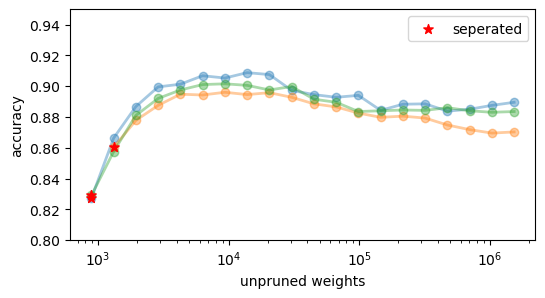
\includegraphics[width=.7\linewidth]{mnist-acc-largest-784-392.png}
    \caption[Performance and Separation on MNIST-Fashion-MNIST]{The performance of three training runs with different seeds. 
    Each line represents one training run, where the hyperparameters are the same.
    The performance where the network separates is indicated by the red star.
    The x-axis shows the number of available/unpruned weights on a logarithmic scale.
    The y-axis shows the accuracy.
    }\label{fig:mnist-acc}
\end{figure}

\begin{figure}
    \centering
    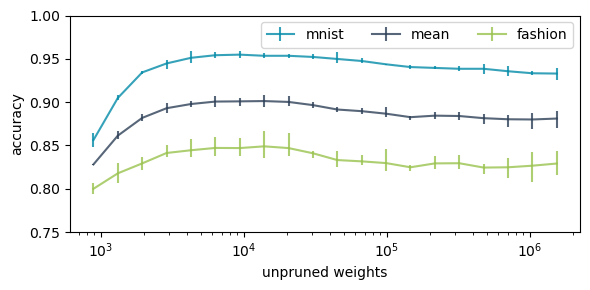
\includegraphics[width=.7\linewidth]{taskwise-acc.png}
    \caption[Taskwise performance]{
        The performance of the separate tasks in the network.
        Each line shows the average, minimum and maximum accuracy of the three repeated training runs.
        The lines show the accuracy of the MNIST task (blue), the Fashion-MNIST task (green) and the average of both (dark blue).
    }\label{fig:taskwise-acc}
\end{figure}

The data shown in figure~\ref{fig:mnist-acc} represents the average accuracy of both tasks.
The data in figure~\ref{fig:taskwise-acc} shows the accuracy of the tasks separately.
Each line is an average of the three runs with different seeds.
The error bars indicate minimum and maximum values.
On the x-axis, the number of active weights is displayed.
On the y-axis, the accuracy is shown.

Since the tasks are not the same, it is to be expected that they do not exhibit the same performance.
The accuracy achieved on the MNIST task is more than $10$~percent higher than on the Fashion MNIST task.
Interestingly, when the number of parameters gets lower, the performance on the MNIST task worsens significantly faster than for the Fashion MNIST task.
The performance of the network is not competitive anymore at the time it separates.
However, the experiments shown here are only preliminary.
The networks indeed separate consistently, and they do far beyond trivial accuracies.
This gives reason to believe, that the separation can be achieved at competitive accuracy with improved hyperparameters or slight adaptations to the training.
This, however, is not pursued in the scope of this thesis.
The separation by itself, at non-trivial accuracy is considered a useful insight into the structure of the network.

\subsection{Connectivity of the input layer}
An interesting finding of \textcite{LTH} was, that certain neurons in the input layer retain significantly more incoming connections than others.
They find this to be the case with winning tickets trained on MNIST and attribute this to the fact that certain pixels of the MNIST dataset do not contain any useful information.
In figure~\ref{fig:mnist-input-variance} the pixel-wise mean and variance of the MNIST dataset is shown.
Since the digits are centered in the image, there is a frame where there is little to no variance and where the values are on average close to zero.

\begin{figure}[!ht] % mnist variance
    \centering 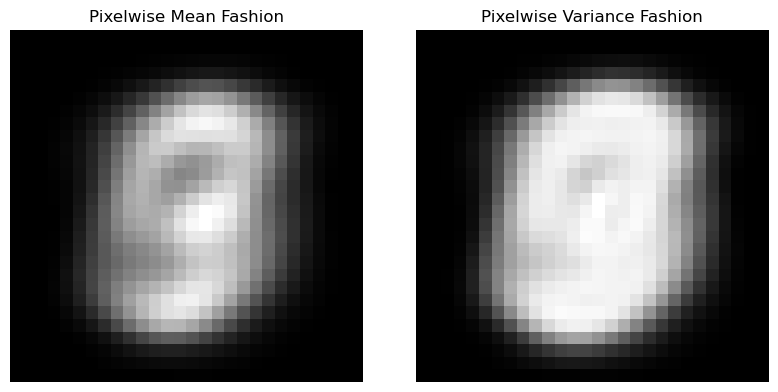
\includegraphics[width=.7\linewidth]{mnist_mean_variance.png}
    \caption[Mean and Variance MNIST]{
    The mean (left) and variance (right) of each pixel in the MNIST dataset
    }\label{fig:mnist-input-variance}
\end{figure}
\begin{figure}[!ht] % fashion variance
    \centering 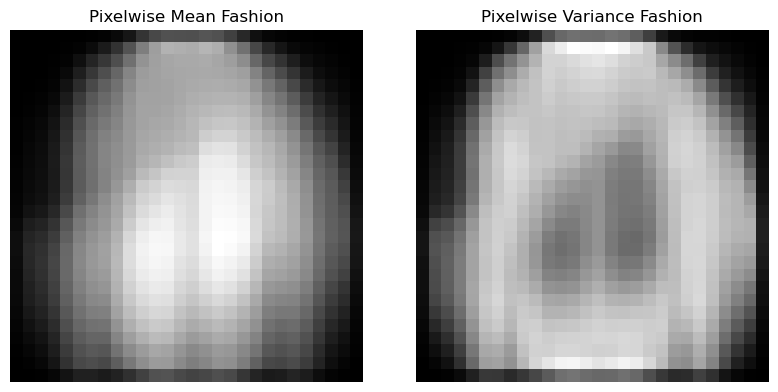
\includegraphics[width=.7\linewidth]{fashion_mnist_mean_variance.png}
    \caption[Mean and Variance Fashion-MNIST]{
        The mean (left) and variance (right) of each pixel in the Fashion-MNIST dataset
        }\label{fig:fashion-input-variance}
\end{figure}

A similar effect is visible with the Fashion MNIST dataset as seen in figure~\ref{fig:fashion-input-variance}.
For the Fashion-MNIST dataset, the frame is notably smaller and there are pixels with significant mean and variance that lie on the outermost pixel row of the image.
For each of the datasets, a neural network with the same architecture as in \autocite{LTH} was used, namely the LeNet architecture with a shape of $(784,300,100,10)$.
The networks were pruned for 18 pruning levels to a pruning target of {$600$}.

Figure~\ref{fig:mnist-heatmap} shows the connectivity to the input layer at different pruning iterations.
The shape of the digits as seen in figure~\ref{fig:mnist-input-variance} is distinctly visible over many pruning levels.
This means that there tend to be more outgoing connections of pixels that are in the high-variance or high-mean area of the image.
At pruning level 11 where only 2 percent of all weights are active, many pixels on the outer frame of the image do not have any connection left.
At iteration 15, most of the pixels on the outer frame have been completely disconnected.
However, there remain some pixels on the outer frame that hold onto the connections, even though they do not carry any information.
This suggests that there is an increased likelihood of disconnecting from pixels with no information.
Due to the probabilistic nature of training and network initialization, there may remain connections to zero-information inputs.

\begin{figure}[!htb] % MNIST attention heatmap
    \centering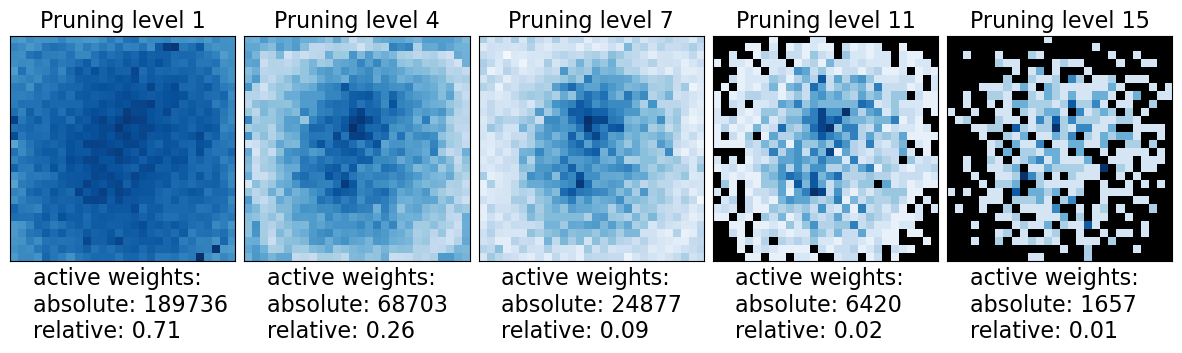
\includegraphics[width=1.\linewidth]{mnist_input_attention_active.png}
    \caption[Pixel connectivity MNIST]{
        Heatmap of the number of outgoing connections of each input pixel of the MNIST dataset, over several pruning levels.
        }\label{fig:mnist-heatmap}
\end{figure}
\begin{figure}[!htb] % Fashion attention heatmap
    \centering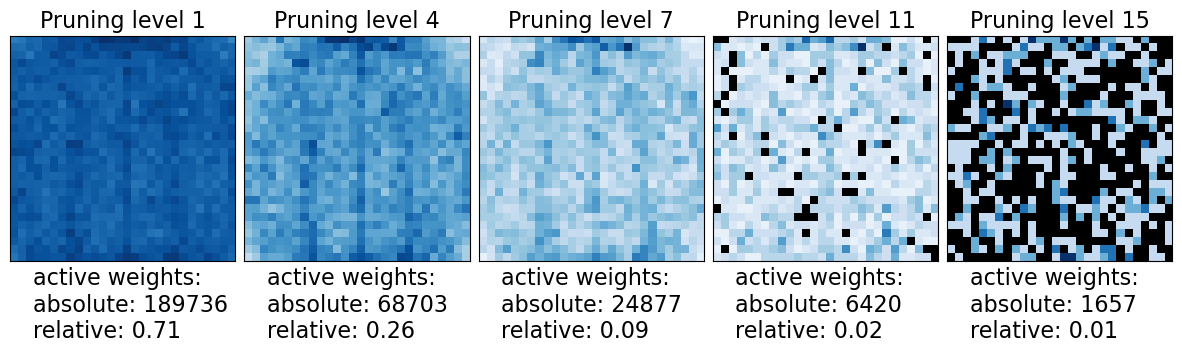
\includegraphics[width=1.\linewidth]{fashion_input_attention_active.png}
    \caption[Pixel connectivity Fashion-MNIST]{
        Heatmap of the number of outgoing connections of each input pixel of the Fashion-MNIST dataset, over several pruning levels.
        }\label{fig:fashion-heatmap}
\end{figure}

Figure~\ref{fig:fashion-heatmap} shows this for the Fashion dataset.
In early iterations, a pattern can be detected that resembles the overall shape of some fashion items.
Further, a line in the center with more connections is visible.
This might be the case because many items have characteristic lines in the center, like trousers, shirts or jackets.
The line is also visible in the mean and variance of the dataset as shown in figure~\ref{fig:fashion-input-variance}.
At pruning levels one, four and seven, the number of connections per pixel shows a similar shape to the mean and variance of the dataset.
At iterations four and seven, there is a horizontal bar of strongly connected pixels in the center of the upper edge of the image. 
This bar is also visible in the pixel-wise variance of the dataset, which indicates a connection between variance and connectivity.
However, with the Fashion dataset, the pattern disappears in later iterations.
At pruning level 11, there is no pattern visible anymore and at iteration 15, many of the center pixels are completely disconnected.

One possible explanation for the clearer pattern in the MNIST dataset is that the different classes are more similar and take up a more compact area in the image, as seen in figure~\ref{fig:mnist-input-variance}.
Also, the performance on the MNIST dataset is better than on the Fashion dataset, with the same hyperparameters.
This might indicate, that the Fashion dataset is harder to learn for the {MLP}, which could also impact the connectivity of the input layer.

%%% old
\begin{figure}[ht] % mnist-fashion-mnist connectivity
    \centering
    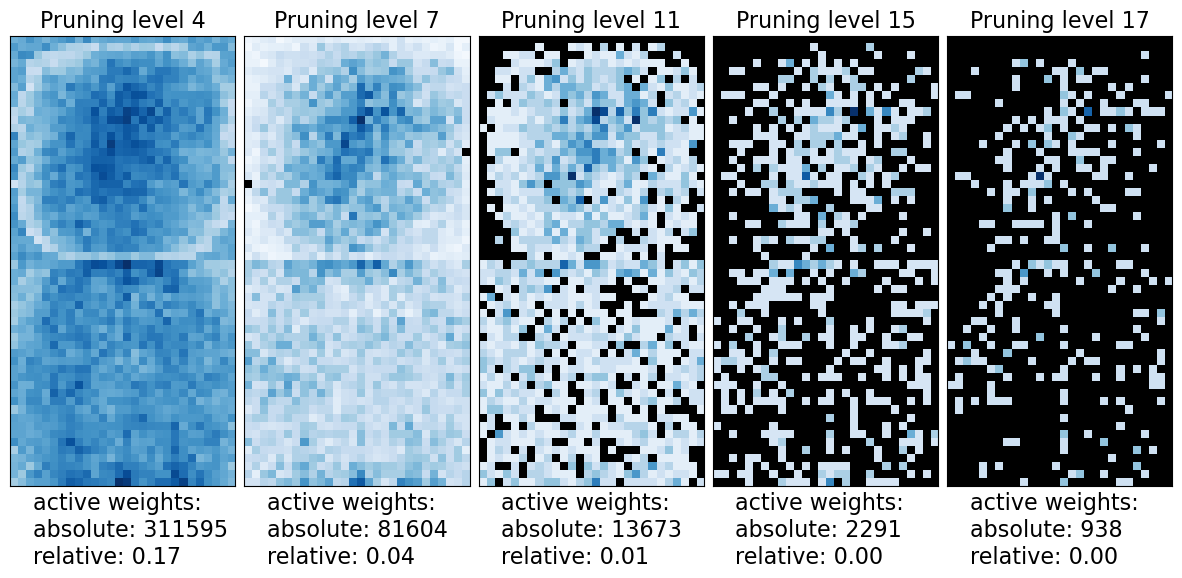
\includegraphics[width=1.\linewidth]{mnist_fashion_mnist_input_attention_active.png}
    \caption[Pixel connectivity MNIST-Fashion-MNIST]{
    Heatmap of the number of outgoing connections of each input pixel of the MNIST-Fashion-MNIST dataset, over several pruning levels.}\label{fig:mnist-fashion-map}
\end{figure}

When examining a training run on the MNIST-Fashion-MNIST set with a network of shape $(1568, 784, 392, 20)$, the same patterns emerge.
In figure~\ref{fig:mnist-fashion-map}, the connectivity on the concatenated dataset is shown.
The images are shown as stacked, where the MNIST image is on top and the Fashion image is on the bottom.
On the MNIST image, the same pattern as before is visible.
In the Fashion image, parts of the pattern are visible but less pronounced.
Given that both tasks are trained at the same time, it might be that the hyperparameters are better suited for MNIST than for Fashion-{MNIST}.
After iteration 17, which is the rightmost image, the network separated.
The connectivity is severely degraded at this point even though the network has an accuracy of $83$ percent at that iteration.
This further advances the point, that the network in this example separated very late in the process.
Improved hyperparameters and training techniques could lead to separation at earlier iterations.